\chapter{Experimental setup}
The experimental setup consists of three scintillators one copper plate and a solenoid arranged as shown in \autoref{fig:setup}

\begin{figure}[H]
    \centering
    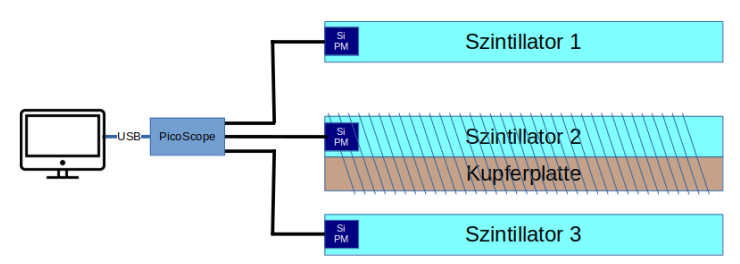
\includegraphics[width=0.5\linewidth]{include/aufbau.png}
    \caption{experimental setup}
    \label{fig:setup}
\end{figure}

The signals from the scintillators are read out with a PicoScope. The copper plate "filters" the Muons, the anti Muons are much less affected by the copper. The solenoid around the second scintillator  makes the spins precess which affects the decay of the muons. 